\documentclass[openacc]{rsproca_new}

\usepackage[T1]{fontenc}
\usepackage[utf8]{inputenc}
\usepackage{lmodern}
\usepackage{microtype}
\usepackage{graphicx}
\usepackage{booktabs}
\usepackage{longtable}
\usepackage{array}
\usepackage{amsmath,amssymb}
\usepackage{threeparttable}
\usepackage{multicol}
\usepackage{url}
\usepackage{csquotes}

\addbibresource{refs_with_doi.bib}

\jname{rsif}
\Journal{J R Soc Interface\ }

\begin{document}

\title{From pelvic geometry to modal compliance: sex-specific deformation pathways in the human pelvic ring}

\author{Michal Kucha\v{r}$^{1,2}$, Alexander Mor\'{a}vek$^{2}$, Niels Hammer$^{3,4}$, Petr Heny\v{s}$^{1}$}

\address{$^{1}$Institute of New Technologies and Applied Informatics, Faculty of Mechatronics, Informatics and Interdisciplinary Studies, Technical University of Liberec, Liberec, Czech Republic\\
$^{2}$Department of Anatomy, Faculty of Medicine in Hradec Kr\'{a}lov\'{e}, Charles University, Hradec Kr\'{a}lov\'{e}, Czech Republic\\
$^{3}$Division of Macroscopic and Clinical Anatomy, Gottfried Schatz Research Center, Medical University of Graz, Graz, Austria\\
$^{4}$Department of Orthopedic and Trauma Surgery, University of Leipzig, Leipzig, Germany; Division of Biomechatronics, Fraunhofer IWU, Dresden, Germany}

\subject{biomechanics, evolutionary anthropology, obstetrics}

\keywords{biomechanics, human pelvis, modal analysis, finite-element modelling, childbirth, allometry, sacroiliac joint}

\corres{Alexander Mor\'{a}vek\\
\email{moravekal@lfhk.cuni.cz}}


\begin{abstract}
Walking, posture and childbirth all depend on the same structure: the pelvic ring. Human pelvic dimorphism is usually judged from static birth-canal measurements, but these dimensions do not show how the ring deforms when loaded. We asked whether sex differences in pelvic function are explained by overall size and static pelvimetry, or by available mechanical deformation pathways. We analysed 278 anatomically standardised lumbopelvic finite-element models built from clinical computed tomography scans. In each model, modal decomposition separated pelvic deformation into a shared, ranked set of pathways, allowing us to compare pathway stiffness, load recruitment and sensitivity to ligamentous and cartilaginous constraints.

Overall pelvic size accounted for much of the baseline stiffness spectrum, confirming a strong size-dependent component. Yet adjustment for size and age did not remove sex differences: male pelves showed approximately 20\% higher adjusted eigenvalues than female pelves in modes~2 and~9. Loading probes showed a common backbone in both sexes during habitual support, whereas inlet opening revealed a different response organisation. Mode~9 was the dominant inlet-opening component in 265 of 278 individuals, but female pelves distributed deformation across a broader coordinated set, with a higher effective number of participating modes than male pelves. The principal inlet-opening pathway was most sensitive to the pubic symphysis and anterior sacroiliac ligamentous constraints. Pelvic dimorphism therefore lies not only in canal shape, but in the organisation of mechanical pathways that balance support with deformation.
\end{abstract}


\maketitle

\begin{multicols}{2}

\section{Introduction}

The human pelvis sits at the intersection of biomechanics, evolutionary anthropology and obstetrics. It must transmit loads between the trunk and lower limbs while also forming the bony boundary of the birth canal. This dual role has often been framed geometrically: selection for efficient bipedalism is assumed to constrain pelvic form, whereas selection for parturition favours canal enlargement \cite{RosenbergTrevathan2002,Trevathan2015,Grunstra2023}. Linear dimensions and canal shape are therefore central to most discussions of pelvic function.

A purely geometric account is incomplete, however, because the pelvis does not behave as a rigid frame. It is a constrained, deformable ring whose response depends on available deformation pathways, the stiffness cost of accessing those pathways and the constraints imposed by the sacroiliac joints (SIJs), pubic symphysis and ligamentous architecture. This distinction matters for both locomotor and obstetric interpretation. Moderately wider hips do not appear to impose a simple locomotor cost \cite{Warrener2015}, while recent syntheses of childbirth evolution emphasise the pelvic floor, connective tissues and broader parturition mechanics rather than bony canal dimensions alone \cite{Pavlicev2020,Haeusler2021,Grunstra2023}. Static pelvimetry remains informative, but it is unlikely to capture the full functional phenotype.

Computational modelling provides a route from anatomy to mechanics, especially when heterogeneous bone material, cartilage and ligaments are represented \cite{Eichenseer2011,Hammer2013,Salo2017,Ramezani2019,HammerKlima2019,Ricci2020,Henys2022}. Dynamic birth simulations and pelvic finite-element studies have shown that mechanical interpretation can extend beyond static canal shape \cite{Fremondiere2022}. Most existing studies, however, are subject-specific or based on small specimen cohorts and therefore do not directly show which mechanical features are shared across individuals and which are primarily allometric \cite{HammerKlima2019,Salo2017,Ramezani2019,DubeCyr2021}.

Here we address this gap using 278 standardised human pelves in anatomical correspondence. Rather than reducing each pelvis to a set of obstetric diameters, we describe the pelvic ring as a repertoire of elastic deformation pathways. This separates two questions that are usually conflated: which pathways are mechanically accessible, and how strongly a given load recruits them.

Our working hypothesis was that sex differences in pelvic mechanics are not reducible to overall size or to any single canal dimension. Instead, scale should set much of the baseline stiffness spectrum, whereas sex should be expressed in selected pathways and in the way load cases distribute response energy across them. We therefore tested three linked expectations: allometry explains a substantial share of modal stiffness variation; selected sex differences persist after adjustment for size and age; and habitual support loads and birth-canal-relevant opening probes recruit different parts of the modal repertoire. Support for these expectations would shift the functional interpretation of pelvic dimorphism from static geometry towards mode-specific compliance within a constrained mechanical ring.


\section{Material and methods}

\subsection{CT-derived cohort in anatomical correspondence}

The analysis used BoneDat, a standardised database of 278 clinical lumbopelvic computed tomography (CT) scans from a Central European cohort spanning adolescence to old age \cite{HenysKuchar2025}. The present dataset comprised 150 female and 128 male individuals aged 16--91 years. Subject selection, segmentation, shape normalisation, template construction, mesh generation and technical validation are reported in the source data descriptor; here we summarise only the elements needed for the mechanical analysis.

The resource provides curated segmentations, diffeomorphic deformation fields, a common reference surface, tetrahedral volumetric meshes and a template model. This allowed every pelvis to be analysed on a shared anatomical domain while preserving individual morphology through subject-specific deformation fields. Because the original scans were acquired without a calibration phantom, mapped material properties are interpreted as cohort-wise relative descriptors rather than direct clinical densitometry. Phantomless internal calibration was used to convert the released Hounsfield-unit values to hydroxyapatite-equivalent density before elastic property assignment.

\subsection{Allometric scale and conventional pelvic dimensions}

The principal size variable was the cube root of total pelvic volume relative to the template reference volume. This gives a whole-pelvis linear scale for a three-dimensional structure and avoids using a single canal diameter as a proxy for body size. We also recorded total surface area, total mass, effective thickness and effective density.

Conventional pelvimetric variables were extracted from the registered cohort for comparison with the mechanical measures. These were anteroposterior inlet diameter (AP), pelvic inlet transverse diameter (PIT), subpubic angle, biacetabular width, biischiadic width, bituberous width, sacral width and iliopectineal eminence width. They were used as anatomical comparators, not as replacements for the modal mechanical descriptors.

\subsection{Finite-element spectrum as accessible deformation pathways}

Each finite-element model started from the same tetrahedral template mesh. The mesh was warped into subject space with the subject-specific BoneDat deformation field, so that corresponding nodes and regions referred to the same anatomy across the cohort while retaining individual pelvic shape. Mechanics were assembled on the mapped reference domain. Bone properties were assigned cell-wise from mapped hydroxyapatite-equivalent density; sacroiliac cartilage and the pubic symphysis were assigned region-wise baseline material properties.

The mechanical model was comparative by design. It used small-deformation, linear isotropic elasticity. Rigid support was imposed by penalty constraints, and the major pelvic ligament groups were represented as linear axial springs attached to corresponding anatomical regions. These choices allowed relative elastic pathway accessibility to be compared across individuals within a common modelling framework.

For each subject, we asked which deformation patterns were easiest to access within this elastic model. This was done by solving the generalised eigenproblem
\begin{equation}
K\phi_{k} = \lambda_{k} M\phi_{k}, \qquad k=1,2,\ldots,10,
\end{equation}
where $K$ is the subject-specific stiffness matrix and $M$ is the numerical inner-product matrix used to normalise and compare displacement fields. The modes are quasi-static deformation patterns, not inertial vibration modes. The eigenvalue $\lambda_k$ is the elastic cost of the corresponding $M$-normalised pattern; lower eigenvalues indicate pathways that are more accessible under the adopted metric.

The analyses use modes~1--10. Mode labels were defined after applying the recorded per-subject reordering vectors from the processing pipeline. This step was needed because nearby low-order eigenpairs can exchange numerical order between subjects; after reordering, a label such as mode~9 denotes the aligned deformation family used in the cohort analysis, not merely the ninth raw solver output. The reordering vectors served only for mode correspondence. Because eigenvectors are sign-indeterminate, arbitrary sign changes do not affect the scalar quantities reported here: eigenvalues, modal energy fractions or sensitivity measures.

Two terms are used throughout the manuscript. \emph{Pathway accessibility} denotes the position of a mode in the stiffness spectrum. \emph{Pathway dominance} denotes how much of a particular load response is carried by that mode after loading is applied.

% NOTE TO AUTHORS: Keep the eigenvalues described as relative modal stiffness/accessibility metrics under the adopted M-normalisation, not as natural frequencies or absolute clinical stiffness values.

\subsection{Mechanical probes and modal participation}

Four static loading scenarios were analysed. Bilateral and unilateral stances represented habitual support mechanics, whereas inlet opening and outlet opening served as probes with obstetric relevance, but not as literal simulations of childbirth. Because full subject-specific probe solves were computationally demanding, these four probe configurations were prepared in FEBio Studio \cite{Maas2017FEBioHistory} and solved once on the population template model.  Anatomically defined template regions were used to prescribe the relevant support constraints and force directions for each scenario, so that all probes were applied to the same reference anatomy.

The resulting template displacement fields were defined on the same reference domain as the subject-specific modes and were then projected onto each subject's modal basis. Thus, variation in modal participation reflects the subject-specific spectrum and modal correspondence, while the applied probe field remains standardised. With $\Phi=[\phi_{1},\ldots,\phi_{10}]$, the participation vector $q$ was obtained from
\begin{equation}
(\Phi^{T}M\Phi)q = \Phi^{T}Mu.
\end{equation}
The modal strain energy associated with each coordinate was then calculated as
\begin{equation}
U_{i}=\frac{1}{2}\lambda_{i}q_{i}^{2}\lVert\phi_{i}\rVert_{M}^{2}, \qquad
\eta_{i}=\frac{U_{i}}{\sum_{j}U_{j}}.
\end{equation}
The fraction $\eta_i$ is the share of the response energy carried by mode $i$ after normalisation over modes~1--10. We also tracked the total response energy retained in these ten modes to check that truncation did not determine the reported patterns.

\subsection{Local sensitivity of ligament and interface constraints}

We next asked which soft-tissue constraints most affected the modal spectrum. For each selected mode, we calculated first-order sensitivities of the eigenvalue to small local changes in ligament stiffness or interface modulus. These local, linearised measures rank how strongly a local stiffening would change the elastic cost of an $M$-normalised deformation pathway.

For a ligament bundle with axial stiffness $EA_{\ell}$, the modal sensitivity was
\[
\frac{\partial \lambda_i}{\partial EA_{\ell}} =
\frac{\phi_i^{T}(\partial K/\partial EA_{\ell})\phi_i}
{\phi_i^{T}M\phi_i}.
\]
The reported value therefore reflects the contribution of axial spring stiffness in that ligament bundle to the eigenvalue of mode $i$.

For cartilage and symphyseal interface regions, the code reported a normalised energy-based sensitivity proxy,
\[
S_{i,R} =
\frac{\mathcal{E}_{i}(R)}
{E_R \phi_i^{T}M\phi_i},
\]
which is proportional under linearisation to $\partial \lambda_i/\partial E_R$. Ligament and interface sensitivities were not compared by raw magnitude because they have different units and arise from different perturbation definitions. Percent contributions were therefore calculated separately within the ligament class and within the interface class.

The sensitivity analysis covered the symphyseal ligament group, anterior SIJ ligaments, posterior SIJ ligaments, interosseous SIJ ligaments, sacrospinous ligaments and sacrotuberous ligaments, together with the sacroiliac cartilage interfaces and pubic symphysis. The primary focus was on modes showing the clearest adjusted sex effects.

\subsection{Statistical analysis}

Sex differences in cohort descriptors were assessed with Welch two-sample $t$-tests. Empirical allometry of surface area, mass and effective density was evaluated with log--log regressions against pelvic scale.

Eigenvalues were analysed on the raw scale whenever formal inference was required. Size-normalised eigenvalues were used only for descriptive summaries in table~\ref{tab:modes} and figure~\ref{fig:eigs}. For these summaries, each mode was normalised to the cohort geometric-mean pelvic scale, $S_0=\exp(\overline{\log S})=0.9568452943$. The mode-specific scaling exponent was estimated from
\begin{equation}
\log(\lambda_{ik,\mathrm{raw}})=a_k+b_k\log(S_i)+c_k\,\mathrm{sex}_i+\varepsilon_i,
\end{equation}
and the descriptive size-normalised value was calculated as
\begin{equation}
\lambda_{ik,\mathrm{scaled}}=\lambda_{ik,\mathrm{raw}}\left(\frac{S_i}{S_0}\right)^{\gamma_k},
\qquad \gamma_k=-b_k.
\end{equation}
For modes~1--10, $\gamma_k$ was 1.382, 1.834, 1.676, 2.393, 2.068, 2.139, 2.346, 2.326, 1.887 and 2.136, respectively.

Adjusted sex effects were estimated from
\begin{equation}
\log(\lambda_{\mathrm{raw}}) \sim \log(\mathrm{scale}) + \mathrm{sex} + \mathrm{age}.
\end{equation}
The sex coefficient was expressed as the percentage difference in eigenvalue for male relative to female pelves. Benjamini--Hochberg false-discovery-rate adjusted $q$-values are reported across the ten mode-wise tests.

To assess the contribution of conventional pelvimetry, we fitted female-only models for modes~9 and~2,
\begin{equation}
\log(\lambda_{\mathrm{raw}}) \sim \log(\mathrm{scale}) + \mathrm{age} + \mathrm{dimension},
\end{equation}
and report the incremental contribution of each dimension as partial $R^2$.

Modal participation fractions were summarised as cohort means because they are compositional quantities. Response concentration was also described by the effective number of participating modes,
\begin{equation}
N_{\mathrm{eff}} = \exp\left(-\sum_i p_i\log p_i\right),
\end{equation}
where $p_i$ is the energy fraction of mode $i$ after normalisation over modes~1--10. Larger values indicate a more distributed modal response.

\section{Results}
\subsection{Cohort differences in scale and pelvic dimensions}

The cohort comprised 278 individuals, including 150 female and 128 male individuals. Age did not differ significantly between the sexes (table~\ref{tab:cohort}). Female pelves had smaller overall scale than male pelves, but larger AP and PIT dimensions, a wider subpubic angle, and greater biischiadic and bituberous widths. Sacral width did not differ significantly between the sexes.

Because scale was defined from total pelvic volume, the volume--scale relation is definitional and is not reported as an empirical allometry. Among the remaining quantities, total surface area scaled sub-isometrically with pelvic scale (slope $=1.684$, $R^2=0.894$), total mass increased with scale (slope $=2.679$, $R^2=0.902$), and effective density declined modestly with scale (slope $=-0.321$, $R^2=0.117$; table~\ref{tab:allometry}).

\subsection{Scale dependence, adjusted sex effects and pelvimetric associations}

Before allometric size normalisation, log pelvic scale was negatively correlated with log eigenvalue for all ten modes (table~\ref{tab:modes} and figure~\ref{fig:eigs}). After normalisation to the cohort geometric-mean scale, the correlation was near zero for modes~1 and~5 and positive for several other modes. The strongest positive scaled correlations were observed for modes~2 and~9.

In models using raw eigenvalues with scale and age as covariates, the largest adjusted sex effects occurred in modes~2 and~9. Male pelves had eigenvalues 20.72\% higher than female pelves in mode~2 and 20.07\% higher in mode~9. Positive adjusted male effects were also present in modes~3, 4, 7, 8 and~10. Mode~1 showed no detectable sex effect, and modes~5 and~6 did not survive the same threshold of evidence (table~\ref{tab:modes}).

In female-only pelvimetry models, AP was the strongest single predictor of mode~9 stiffness after adjustment for scale and age (partial $R^2=0.239$, $p=3.04 \times 10^{-10}$), followed by PIT (partial $R^2=0.127$, $p=8.82 \times 10^{-6}$). Iliopectineal eminence width and sacral width showed similar but smaller contributions (table~\ref{tab:pelvimetry} and figure~\ref{fig:pelvimetry}). These significant inlet-related associations were negative, indicating lower mode~9 eigenvalues with larger AP, PIT, iliopectineal eminence width or sacral width; subpubic angle showed a smaller positive association. For mode~2, the largest partial $R^2$ was observed for bituberous width (partial $R^2=0.102$, $p=7.80 \times 10^{-5}$), followed by PIT, biischiadic width and biacetabular width, all with negative coefficients. No pelvimetric variable had a partial $R^2$ above 0.239 for either mode.

\subsection{Modal participation under support and opening probes}

Under bilateral stance, mode~2 accounted for most of the response in both sexes (84.6\% in female pelves and 84.5\% in male pelves; table~\ref{tab:loadcases}). Under unilateral stance, modes~1--3 together accounted for 92.7\% of the response in female pelves and 91.7\% in male pelves. Sex differences in support-loading participation fractions were small in comparison with the dominant mode contributions.

Under inlet opening, mode~9 had the largest response fraction in 265 of 278 subjects. The mean mode~9 fraction was 46.4\% in female pelves and 52.5\% in male pelves. Female pelves had greater mean participation of mode~4 than male pelves (18.2\% versus 6.0\%), whereas mode~8 contributed substantially in both sexes (15.3\% and 18.1\%). The effective number of participating modes was higher in female than male pelves for inlet opening ($N_{\mathrm{eff}}=4.53\pm0.71$ versus $4.04\pm0.76$; Welch $p=8.05\times10^{-8}$).

Under outlet opening, mode~5 had the largest mean fraction in both sexes (40.7\% in female pelves and 39.2\% in male pelves). Female pelves had greater concurrent participation of mode~9 (16.1\% versus 12.4\%), whereas male pelves had greater participation of mode~6 (22.1\% versus 17.8\%). Representative load applications and modal deformation patterns are shown in figure~\ref{fig:workflow}.

\subsection{Soft-tissue sensitivity profiles across modes}

Soft-tissue sensitivity profiles were compared for modes~2, 3, 4, 8 and~9, with left and right structures averaged for bilateral tissues (table~\ref{tab:sensitivity}). Ligament and interface results are reported as separate within-class rankings because the two sensitivity measures have different units and perturbation definitions.

Among the analysed modes, total interface sensitivity was highest in mode~9, followed by mode~8. In mode~9, the SIJ cartilage interface accounted for 59.2\% of interface sensitivity and the pubic symphysis interface for 40.8\%. Mode~8 interface sensitivity was concentrated mainly at the SIJ cartilage interface (93.5\%).

Total ligament sensitivity was also highest in mode~9. Within the mode~9 ligament profile, the largest contribution came from the symphyseal ligament group (59.3\%), followed by the anterior SIJ ligaments (25.3\%) and interosseous SIJ ligaments (13.1\%). Mode~8 had a lower total ligament sensitivity and was dominated by anterior SIJ ligaments (57.7\%). Modes~2--4 had lower total ligament sensitivities, with contributions mainly from the anterior SIJ and symphyseal ligament groups.

\section{Discussion}
\subsection{A selective mechanical phenotype of pelvic dimorphism}

Read together, the results shift pelvic dimorphism from a purely geometric description to a mechanical one. The cohort showed the expected sex differences in inlet dimensions, subpubic angle and outlet-related breadths, but those differences were not a simple uniform rescaling of the pelvis. The modal analysis adds the missing mechanical layer: scale explained much of the background spectrum, yet selected deformation pathways remained sexually structured after scale and age were accounted for.

This selectivity is central. If pelvic dimorphism were only an effect of size, the adjusted modal spectrum should have been largely neutral. Instead, modes~2 and~9 remained the clearest sex-biased pathways, with additional effects in several neighbouring modes. The result is therefore not that the whole female pelvis is globally softer, nor that the whole male pelvis is globally stiffer. Rather, sex differences are concentrated in particular deformation families within a shared pelvic-ring architecture.

\subsection{Static diameters are predictors, not the mechanical phenotype itself}

The pelvimetry results show why geometry remains important but incomplete. AP and PIT were related to mode~9, and bituberous width was related to mode~2, so conventional dimensions clearly carry mechanical information. At the same time, no single dimension captured most of the modal variance. A diameter describes bony space along one line; an eigenmode reflects how the full ring deforms under the combined influence of shape, bone distribution, cartilage interfaces and ligamentous constraints.

This distinction is especially important for obstetric interpretation. Static pelvimetry can describe the canal, but it cannot by itself describe how the pelvic ring accesses deformation pathways when loaded. The present modal approach therefore does not replace pelvimetry. It explains why similar dimensions need not imply identical compliance, and why mechanically relevant compliance may be concentrated in specific deformation pathways rather than expressed as global pelvic softening.

\subsection{Shared support, selective opening and anterior constraint}

The load projections clarify how these pathways are used under standardised probe fields. Bilateral and unilateral stance recruited a common low-order support pattern in both sexes, whereas inlet opening exposed a different organisation of response energy. Mode~9 was the largest inlet-opening component in almost all subjects, but male pelves concentrated more of the response into this one mode. Female pelves showed a higher effective number of participating modes, indicating that the inlet-opening response was spread across a broader set of coordinated pathways.

This is a more precise interpretation than saying that female pelves are simply more compliant. The difference lies in the organisation of compliance: support mechanics remain broadly shared, while opening probes redistribute the response in a sex-specific way. Outlet opening supports the same view because mode~5 dominated in both sexes, yet female pelves retained greater concurrent mode~9 participation. Inlet and outlet mechanics therefore appear to be overlapping expressions of one constrained ring rather than independent modules.

The sensitivity results provide the anatomical link. Mode~9 combined the highest interface sensitivity with a ligament profile dominated by the symphyseal ligament group, anterior SIJ ligaments and interosseous SIJ ligaments. This pattern is consistent with clinical and anatomical evidence that pregnancy- and childbirth-related mobility is concentrated around the pubic symphysis and anteriorly located sacroiliac constraints \cite{Damen2001,Pires2015,Cicek2015,Fiani2021}, while posterior ligaments such as the sacrospinous and sacrotuberous ligaments contribute importantly to posterior pelvic stability \cite{Hammer2019,Aldabe2019}. The present results extend that interpretation by suggesting that soft-tissue influence on pelvic mechanics may be mode-selective rather than global.

\subsection{Clinical relevance: pathway-selective laxity as a testable mechanism}

Clinically, these findings provide a mechanistic vocabulary for conditions often discussed under the broad term pelvic laxity. Pregnancy-related pelvic girdle pain, symphyseal separation and SIJ-related dysfunction can involve different anatomical regions and different loading tasks \cite{Damen2001,Vleeming2012,Kiapour2019,Stolarczyk2021}. In the present models, the same soft-tissue constraints did not contribute uniformly to all modes. Anterior SIJ and symphyseal constraints had disproportionate influence on the inlet-opening pathway, while support loading remained organised around a shared low-order backbone.

This suggests a clinically testable hypothesis: changes in ligamentous or cartilaginous properties during pregnancy and parturition may selectively alter access to particular deformation pathways rather than simply increasing global pelvic mobility. A small change in symphyseal or anterior SIJ constraint could increase access to an opening pathway without equivalently compromising stance mechanics. Future work can test this pathway-level interpretation by combining pregnancy status, pain phenotype, dynamic imaging, fetal presentation and delivery outcome with subject-specific mechanical models.

\subsection{Scope of the obstetric interpretation and limitations}

The claim of the present study is focused: both sexes share a support-oriented low-order repertoire, but differ in the accessibility and recruitment of selected deformation pathways, especially the inlet-opening pathway represented by mode~9. In this framework, the relevant phenotype is not pelvic size, canal shape or laxity alone, but the organisation of mode-specific compliance within a constrained ring.

Several limitations define the scope of this interpretation. The cohort represents a Central European clinical CT sample and was not linked to obstetric outcomes. The finite-element formulation captures the small-deformation elastic regime, uses phantomless CT-derived material descriptors and omits subject-specific nonlinear tissue behaviour. In addition, the mechanical probe fields were solved on the population template for computational tractability and then projected onto subject-specific modal bases; this standardises the probes but does not capture individual variation in boundary-condition response.

\section{Conclusion}

In this population-scale, correspondence-preserving analysis of 278 human pelves, allometry explained much of the baseline accessibility of deformation pathways but did not exhaust pelvic mechanics. After adjustment for scale and age, strong sex differences remained in selected modes, especially modes~2 and~9. Habitual support scenarios relied on a shared low-order modal backbone in both sexes, whereas inlet- and outlet-opening probes revealed sex-specific reorganisation of compliance. The principal inlet-opening pathway was most sensitive to the pubic symphysis, anterior SIJ ligaments and sacroiliac cartilage interfaces.

The key novelty is therefore not the rediscovery of pelvic dimorphism, but the demonstration that pelvic function is organised through mode-specific compliance that cannot be reduced to size or to any single obstetric diameter. Within the limits of the present elastic modelling framework, female pelves in this cohort are best interpreted as pathway-selective compliant rings: structures that preserve ordinary support while maintaining selectively accessible, anteriorly constrained pathways relevant to childbirth mechanics and pelvic-ring clinical disorders.

\section*{Ethics}

This study used retrospectively acquired clinical CT data released through the BoneDat resource. According to the BoneDat dataset documentation, the study was approved by the Ethics Committee of University Hospital Hradec Kr\'{a}lov\'{e} (Ref: 202411IO3P).

\section*{Data accessibility}

The BoneDat source morphology dataset is available through the published data descriptor \cite{HenysKuchar2025}. Derived statistical tables, mode-correspondence metadata, figure-generation scripts and supplementary processing code are available at: [repository DOI or URL to be inserted before submission].

\section*{Authors' contributions}

P.H. and M.K. conceptualised the study. P.H. and M.K. performed the computational workflow. P.H., M.K. and A.M. analysed the data. P.H., M.K. and A.M. drafted the manuscript. N.H. contributed anatomical and biomechanical interpretation and critically revised the text. All authors approved the final version.

\section*{Competing interests}

The authors declare no competing interests.

\section*{Funding}
Czech Science Foundation Grant No. 24-10862S supported the research.
\end{multicols}

\begin{table}[p]
\centering
\caption{Cohort summary and static pelvic measures. Values are mean $\pm$ s.d. $p$-values are Welch two-sample $t$-tests (female versus male). AP, anteroposterior inlet diameter; PIT, pelvic inlet transverse diameter.}
\label{tab:cohort}
\begin{tabular}{lccc}
\toprule
Measure & Female $(n=150)$ & Male $(n=128)$ & $p$ \\
\midrule
Age (years) & $53.4 \pm 19.7$ & $54.5 \pm 18.9$ & 0.617 \\
Scale & $0.925 \pm 0.045$ & $0.998 \pm 0.045$ & $6.51 \times 10^{-32}$ \\
Effective density & $1.341 \pm 0.079$ & $1.321 \pm 0.074$ & 0.028 \\
AP (mm) & $121.0 \pm 10.0$ & $112.3 \pm 9.1$ & $4.63 \times 10^{-13}$ \\
PIT (mm) & $134.9 \pm 8.6$ & $127.7 \pm 7.6$ & $2.88 \times 10^{-12}$ \\
Subpubic angle (deg) & $85.8 \pm 6.1$ & $69.1 \pm 5.3$ & $7.30 \times 10^{-71}$ \\
Biacetabular width (mm) & $129.1 \pm 8.2$ & $122.0 \pm 7.2$ & $2.94 \times 10^{-13}$ \\
Biischiadic width (mm) & $109.9 \pm 7.1$ & $97.7 \pm 7.1$ & $9.40 \times 10^{-35}$ \\
Bituberous width (mm) & $136.5 \pm 8.3$ & $127.3 \pm 7.5$ & $3.03 \times 10^{-19}$ \\
Sacral width (mm) & $116.7 \pm 5.7$ & $117.5 \pm 6.5$ & 0.327 \\
Iliopectineal eminence width (mm) & $106.2 \pm 7.0$ & $97.9 \pm 6.0$ & $1.90 \times 10^{-22}$ \\
\bottomrule
\end{tabular}
\end{table}

\begin{table}[p]
\centering
\caption{Empirical allometric scaling of geometric and material-derived quantities. Slopes are from log--log regressions against pelvic scale. Total volume is omitted because pelvic scale was defined from volume.}
\label{tab:allometry}
\begin{tabular}{lccc}
\toprule
Outcome versus scale & Slope & $p$ & $R^2$ \\
\midrule
Total surface & 1.684 & $2.53 \times 10^{-136}$ & 0.894 \\
Total mass & 2.679 & $2.58 \times 10^{-141}$ & 0.902 \\
Effective density & $-0.321$ & $5.07 \times 10^{-9}$ & 0.117 \\
\bottomrule
\end{tabular}
\end{table}

\begin{table}[p]
\centering
\caption{Mode-wise scale dependence and adjusted sex effects (modes~1--10). Correlations are Pearson's $r$ between $\log(\mathrm{scale})$ and $\log(\lambda)$ for unscaled and allometrically size-normalised eigenvalues. Scaled values were calculated as $\lambda_{\mathrm{scaled}}=\lambda_{\mathrm{raw}}(S/S_0)^{\gamma_k}$, where $S_0=0.9568452943$ and $\gamma_k$ was estimated separately for each mode from a sex-adjusted log--log scaling model. Adjusted sex effect is the percent change in eigenvalue in men relative to women from models of the form $\log(\lambda_{\mathrm{raw}}) \sim \log(\mathrm{scale}) + \mathrm{sex} + \mathrm{age}$. $q$ values are Benjamini--Hochberg adjusted across the ten mode-wise sex tests.}
\label{tab:modes}
\scriptsize
\setlength{\tabcolsep}{3pt}
\begin{tabular}{ccccccc}
\toprule
Mode & $r$ (unscaled) & $p$ & $r$ (scaled) & $p$ & Sex effect & $q_{\mathrm{sex}}$ \\
\midrule
1  & $-0.461$ & $4.96 \times 10^{-16}$ & 0.009 & 0.876 & $+0.85\%$ ($p=0.734$) & 0.734 \\
2  & $-0.331$ & $1.52 \times 10^{-8}$  & 0.374 & $1.20 \times 10^{-10}$ & $+20.72\%$ ($p=2.62 \times 10^{-18}$) & $1.31 \times 10^{-17}$ \\
3  & $-0.467$ & $1.82 \times 10^{-16}$ & 0.233 & $8.84 \times 10^{-5}$  & $+11.23\%$ ($p=1.80 \times 10^{-7}$) & $3.60 \times 10^{-7}$ \\
4  & $-0.509$ & $1.04 \times 10^{-19}$ & 0.273 & $3.70 \times 10^{-6}$  & $+15.90\%$ ($p=4.81 \times 10^{-9}$) & $1.20 \times 10^{-8}$ \\
5  & $-0.607$ & $2.16 \times 10^{-29}$ & $-0.043$ & 0.480 & $-4.18\%$ ($p=0.106$) & 0.118 \\
6  & $-0.684$ & $9.25 \times 10^{-40}$ & 0.079 & 0.188 & $+3.39\%$ ($p=0.097$) & 0.118 \\
7  & $-0.778$ & $1.44 \times 10^{-57}$ & 0.179 & $2.76 \times 10^{-3}$  & $+5.13\%$ ($p=9.70 \times 10^{-4}$) & $1.39 \times 10^{-3}$ \\
8  & $-0.579$ & $2.59 \times 10^{-26}$ & 0.304 & $2.44 \times 10^{-7}$  & $+14.45\%$ ($p=4.88 \times 10^{-11}$) & $1.63 \times 10^{-10}$ \\
9  & $-0.369$ & $2.06 \times 10^{-10}$ & 0.388 & $1.97 \times 10^{-11}$ & $+20.07\%$ ($p=8.15 \times 10^{-20}$) & $8.15 \times 10^{-19}$ \\
10 & $-0.630$ & $4.28 \times 10^{-32}$ & 0.218 & $2.56 \times 10^{-4}$  & $+8.66\%$ ($p=1.43 \times 10^{-5}$) & $2.38 \times 10^{-5}$ \\
\bottomrule
\end{tabular}
\end{table}

\begin{table}
\caption{Female-only associations between static pelvic dimensions and modal stiffness for the two most sex-biased modes. Values are partial $R^2$ and $p$ for models of the form $\log(\lambda_{\mathrm{raw}}) \sim \log(\mathrm{scale}) + \mathrm{age} + \mathrm{dimension}$.}
\label{tab:pelvimetry}
\centering
\begin{tabular}{lcccc}
\toprule
& \multicolumn{2}{c}{Mode 9} & \multicolumn{2}{c}{Mode 2} \\
\cmidrule(lr){2-3}\cmidrule(lr){4-5}
Dimension & Partial $R^2$ & $p$ & Partial $R^2$ & $p$ \\
\midrule
AP & 0.239 & $3.04 \times 10^{-10}$ & 0.002 & 0.628 \\
PIT & 0.127 & $8.82 \times 10^{-6}$ & 0.079 & $5.18 \times 10^{-4}$ \\
Iliopectineal eminence width & 0.114 & $2.83 \times 10^{-5}$ & 0.027 & 0.046 \\
Sacral width & 0.114 & $2.70 \times 10^{-5}$ & 0.023 & 0.063 \\
Biacetabular width & 0.012 & 0.188 & 0.069 & $1.23 \times 10^{-3}$ \\
Biischiadic width & 0.033 & 0.027 & 0.077 & $6.43 \times 10^{-4}$ \\
Bituberous width & 0.021 & 0.082 & 0.102 & $7.80 \times 10^{-5}$ \\
Subpubic angle & 0.032 & 0.029 & 0.011 & 0.197 \\
\bottomrule
\end{tabular}
\end{table}

\begin{table}[p]
\centering
\caption{Mean modal participation fractions (\%) for template-based loading probes after normalisation over modes~1--10. Values are descriptive cohort means for compositional modal fractions. The first ten modes retained $>99\%$ of total response energy in the support scenarios and $91$--$99\%$ in the inlet and outlet probes. The additional LAB phase-3 output present in the working files was not analysed here.}
\label{tab:loadcases}
\begin{tabular}{llrrrrrrrrrr}
\toprule
Scenario & Sex & M1 & M2 & M3 & M4 & M5 & M6 & M7 & M8 & M9 & M10 \\
\midrule
Bilateral stance & Female & 0.4 & 84.6 & 0.1 & 7.3 & 4.0 & 1.0 & 0.1 & 1.3 & 1.1 & 0.1 \\
Bilateral stance & Male   & 0.6 & 84.5 & 0.1 & 4.9 & 4.2 & 1.6 & 0.2 & 2.9 & 0.8 & 0.1 \\
Unilateral stance & Female & 39.6 & 37.8 & 15.3 & 2.6 & 1.5 & 1.2 & 0.2 & 0.5 & 0.7 & 0.6 \\
Unilateral stance & Male   & 40.4 & 37.2 & 14.1 & 1.9 & 1.4 & 2.3 & 0.2 & 1.0 & 0.7 & 0.9 \\
Inlet opening & Female & 0.6 & 4.4 & 4.5 & 18.2 & 3.8 & 1.6 & 1.0 & 15.3 & 46.4 & 4.3 \\
Inlet opening & Male   & 0.7 & 3.1 & 5.1 & 6.0 & 3.4 & 1.5 & 1.1 & 18.1 & 52.5 & 8.5 \\
Outlet opening & Female & 0.4 & 2.6 & 0.4 & 15.7 & 40.7 & 17.8 & 0.9 & 3.8 & 16.1 & 1.6 \\
Outlet opening & Male   & 0.4 & 2.4 & 1.1 & 16.4 & 39.2 & 22.1 & 1.2 & 2.8 & 12.4 & 2.1 \\
\bottomrule
\end{tabular}
\end{table}

\begin{table}[p]
\centering
\caption{Soft-tissue sensitivity profile for modes~2, 3, 4, 8 and~9. Values are cohort means. Percentages indicate the contribution of each structure to the total sensitivity of the corresponding mode within the same tissue class. Left and right structures were averaged for bilateral tissues before reporting. Interface and ligament sensitivities are reported together for completeness, but percentages were calculated separately within each class.}
\label{tab:sensitivity}
\scriptsize
\setlength{\tabcolsep}{3pt}
\renewcommand{\arraystretch}{1.25}
\resizebox{0.96\linewidth}{!}{%
\begin{tabular}{lccccc}
\toprule
Structure & Mode 2 & Mode 3 & Mode 4 & Mode 8 & Mode 9 \\
\midrule
\multicolumn{6}{l}{\textit{Interface sensitivity}} \\

SIJ cartilage interface &
$2.10 \times 10^{-4}$ (95.7\%) &
$2.69 \times 10^{-4}$ (40.3\%) &
$6.08 \times 10^{-4}$ (67.6\%) &
$2.01 \times 10^{-3}$ (93.5\%) &
$3.00 \times 10^{-3}$ (59.2\%) \\

Pubic symphysis interface &
$9.45 \times 10^{-6}$ (4.3\%) &
$3.99 \times 10^{-4}$ (59.7\%) &
$2.92 \times 10^{-4}$ (32.4\%) &
$1.39 \times 10^{-4}$ (6.5\%) &
$2.07 \times 10^{-3}$ (40.8\%) \\

\textit{Total interface sensitivity} &
$2.19 \times 10^{-4}$ (100\%) &
$6.68 \times 10^{-4}$ (100\%) &
$9.00 \times 10^{-4}$ (100\%) &
$2.15 \times 10^{-3}$ (100\%) &
$5.07 \times 10^{-3}$ (100\%) \\

\midrule
\multicolumn{6}{l}{\textit{Ligament sensitivity}} \\

Symphyseal ligament group &
$2.12 \times 10^{-9}$ (5.7\%) &
$2.96 \times 10^{-8}$ (30.4\%) &
$7.56 \times 10^{-8}$ (38.3\%) &
$7.86 \times 10^{-8}$ (15.8\%) &
$1.09 \times 10^{-6}$ (59.3\%) \\

Anterior SIJ ligaments &
$2.59 \times 10^{-8}$ (69.2\%) &
$4.68 \times 10^{-8}$ (48.0\%) &
$8.38 \times 10^{-8}$ (42.4\%) &
$2.87 \times 10^{-7}$ (57.7\%) &
$4.64 \times 10^{-7}$ (25.3\%) \\

Interosseous SIJ ligaments &
$4.68 \times 10^{-11}$ (0.1\%) &
$3.75 \times 10^{-10}$ (0.4\%) &
$1.20 \times 10^{-8}$ (6.1\%) &
$2.20 \times 10^{-8}$ (4.4\%) &
$2.40 \times 10^{-7}$ (13.1\%) \\

Posterior SIJ ligaments &
$2.87 \times 10^{-9}$ (7.7\%) &
$7.06 \times 10^{-9}$ (7.2\%) &
$2.05 \times 10^{-8}$ (10.4\%) &
$3.76 \times 10^{-8}$ (7.6\%) &
$1.27 \times 10^{-8}$ (0.7\%) \\

Sacrospinous ligaments &
$5.85 \times 10^{-9}$ (15.6\%) &
$1.23 \times 10^{-8}$ (12.6\%) &
$4.76 \times 10^{-9}$ (2.4\%) &
$1.75 \times 10^{-8}$ (3.5\%) &
$6.57 \times 10^{-9}$ (0.4\%) \\

Sacrotuberous ligaments &
$6.49 \times 10^{-10}$ (1.7\%) &
$1.27 \times 10^{-9}$ (1.3\%) &
$8.90 \times 10^{-10}$ (0.5\%) &
$5.48 \times 10^{-8}$ (11.0\%) &
$2.37 \times 10^{-8}$ (1.3\%) \\

\bottomrule
\end{tabular}%
}
\end{table}

\begin{figure}[p]
\centering
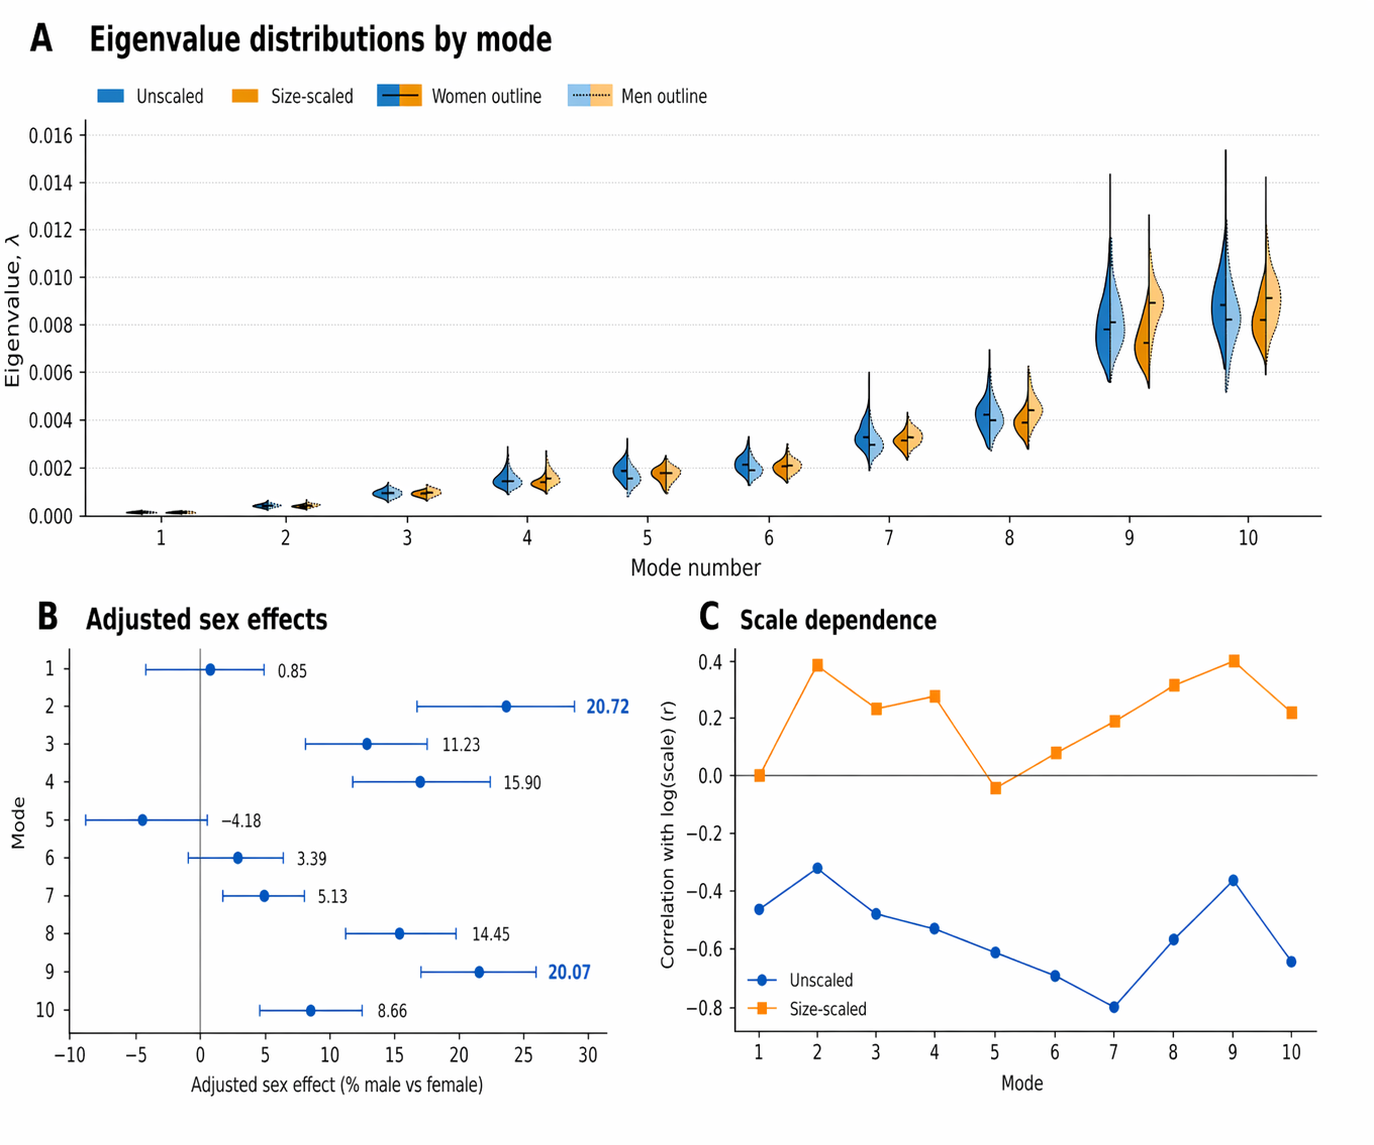
\includegraphics[width=0.95\linewidth]{Figures/violin_final.png}
\caption{Mode-wise eigenvalue distributions, adjusted sex effects and scale dependence. (\textbf{A}) Distributions of eigenvalues $\lambda$ for modes~1--10 before and after descriptive allometric size normalisation to the cohort geometric-mean scale ($\lambda_{\mathrm{scaled}}=\lambda_{\mathrm{raw}}(S/S_0)^{\gamma_k}$). (\textbf{B}) Adjusted sex effects for each mode, expressed as the percentage difference in eigenvalue in men relative to women after adjustment for pelvic scale and age; points denote estimates and horizontal bars denote the corresponding confidence intervals. (\textbf{C}) Mode-wise Pearson correlations between $\log(\mathrm{scale})$ and $\log(\lambda)$ before and after size normalisation.}
\label{fig:eigs}
\end{figure}

\begin{figure}[p]
\centering
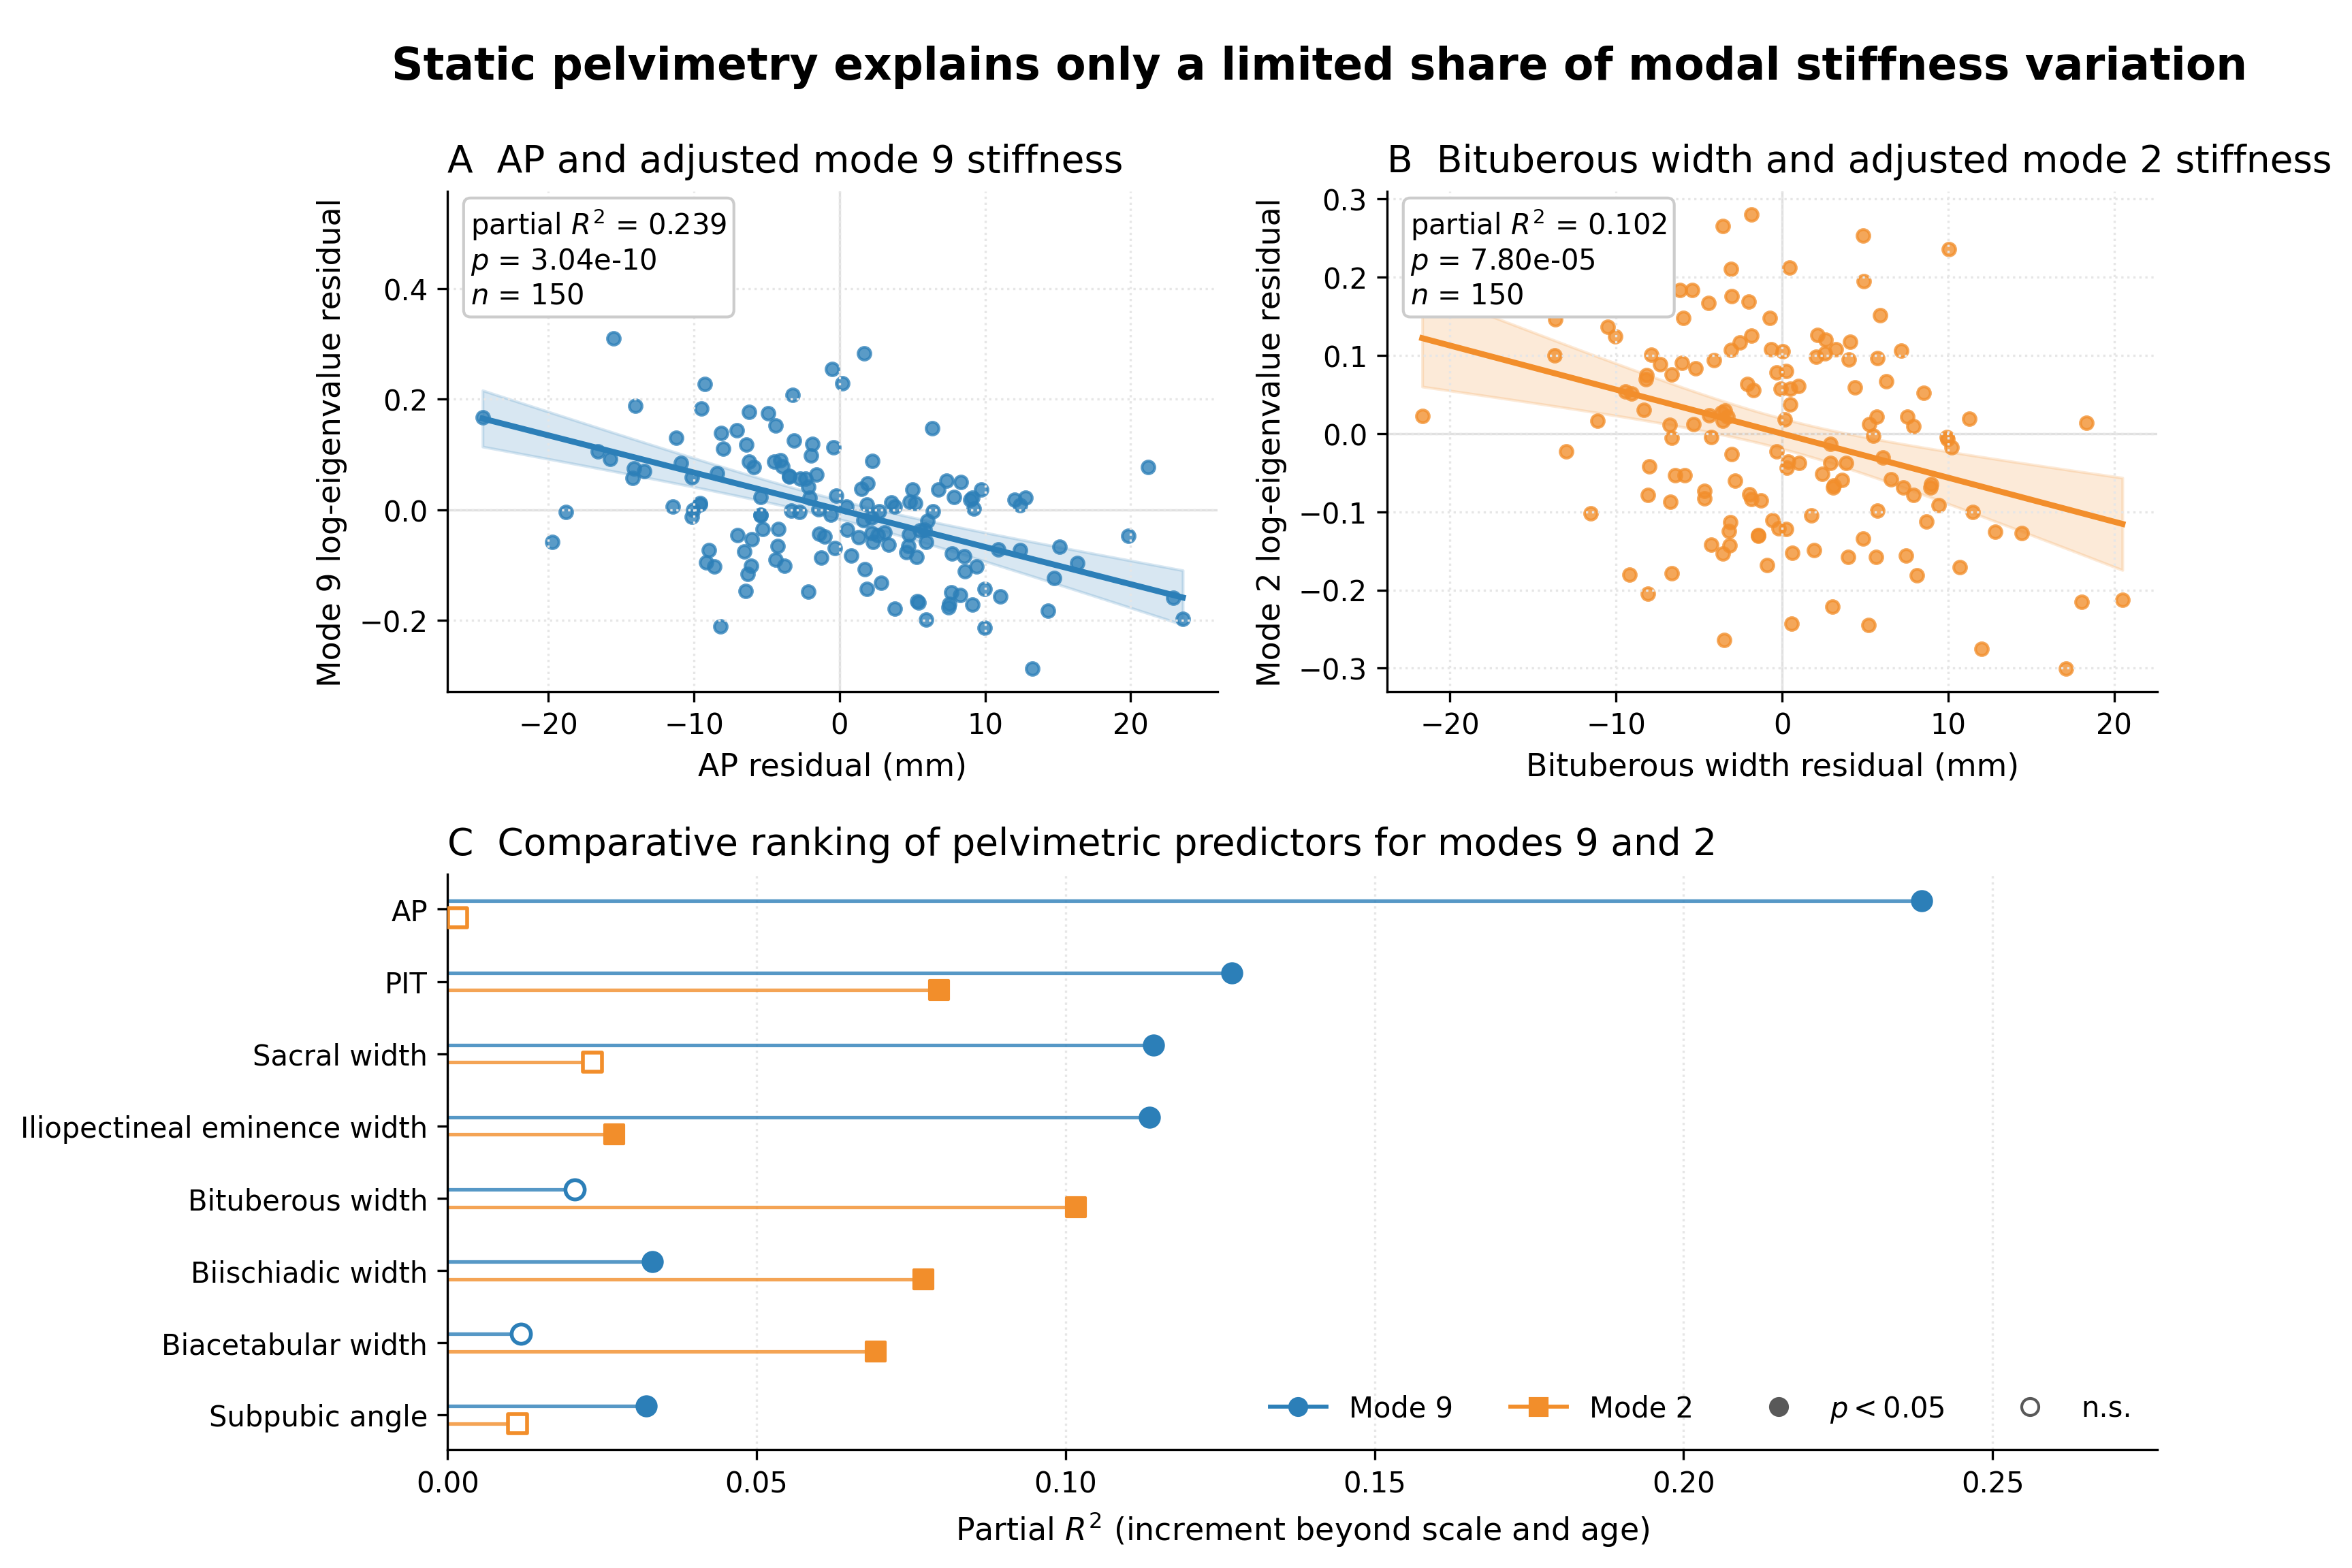
\includegraphics[width=0.95\linewidth]{Figures/Fig5_pelvimetry.png}
\caption{(A) Added-variable plot showing the adjusted association between the anteroposterior inlet diameter (AP) and mode~9 stiffness, expressed as the log-transformed eigenvalue. (B) Added-variable plot showing the adjusted association between bituberous width and mode~2 stiffness. (C) Comparative ranking of pelvimetric predictors for modes~9 and~2, expressed as partial $R^2$ values, i.e.\ the incremental proportion of variance explained by each pelvimetric variable beyond scale and age.}
\label{fig:pelvimetry}
\end{figure}

\begin{figure}[p]
\centering
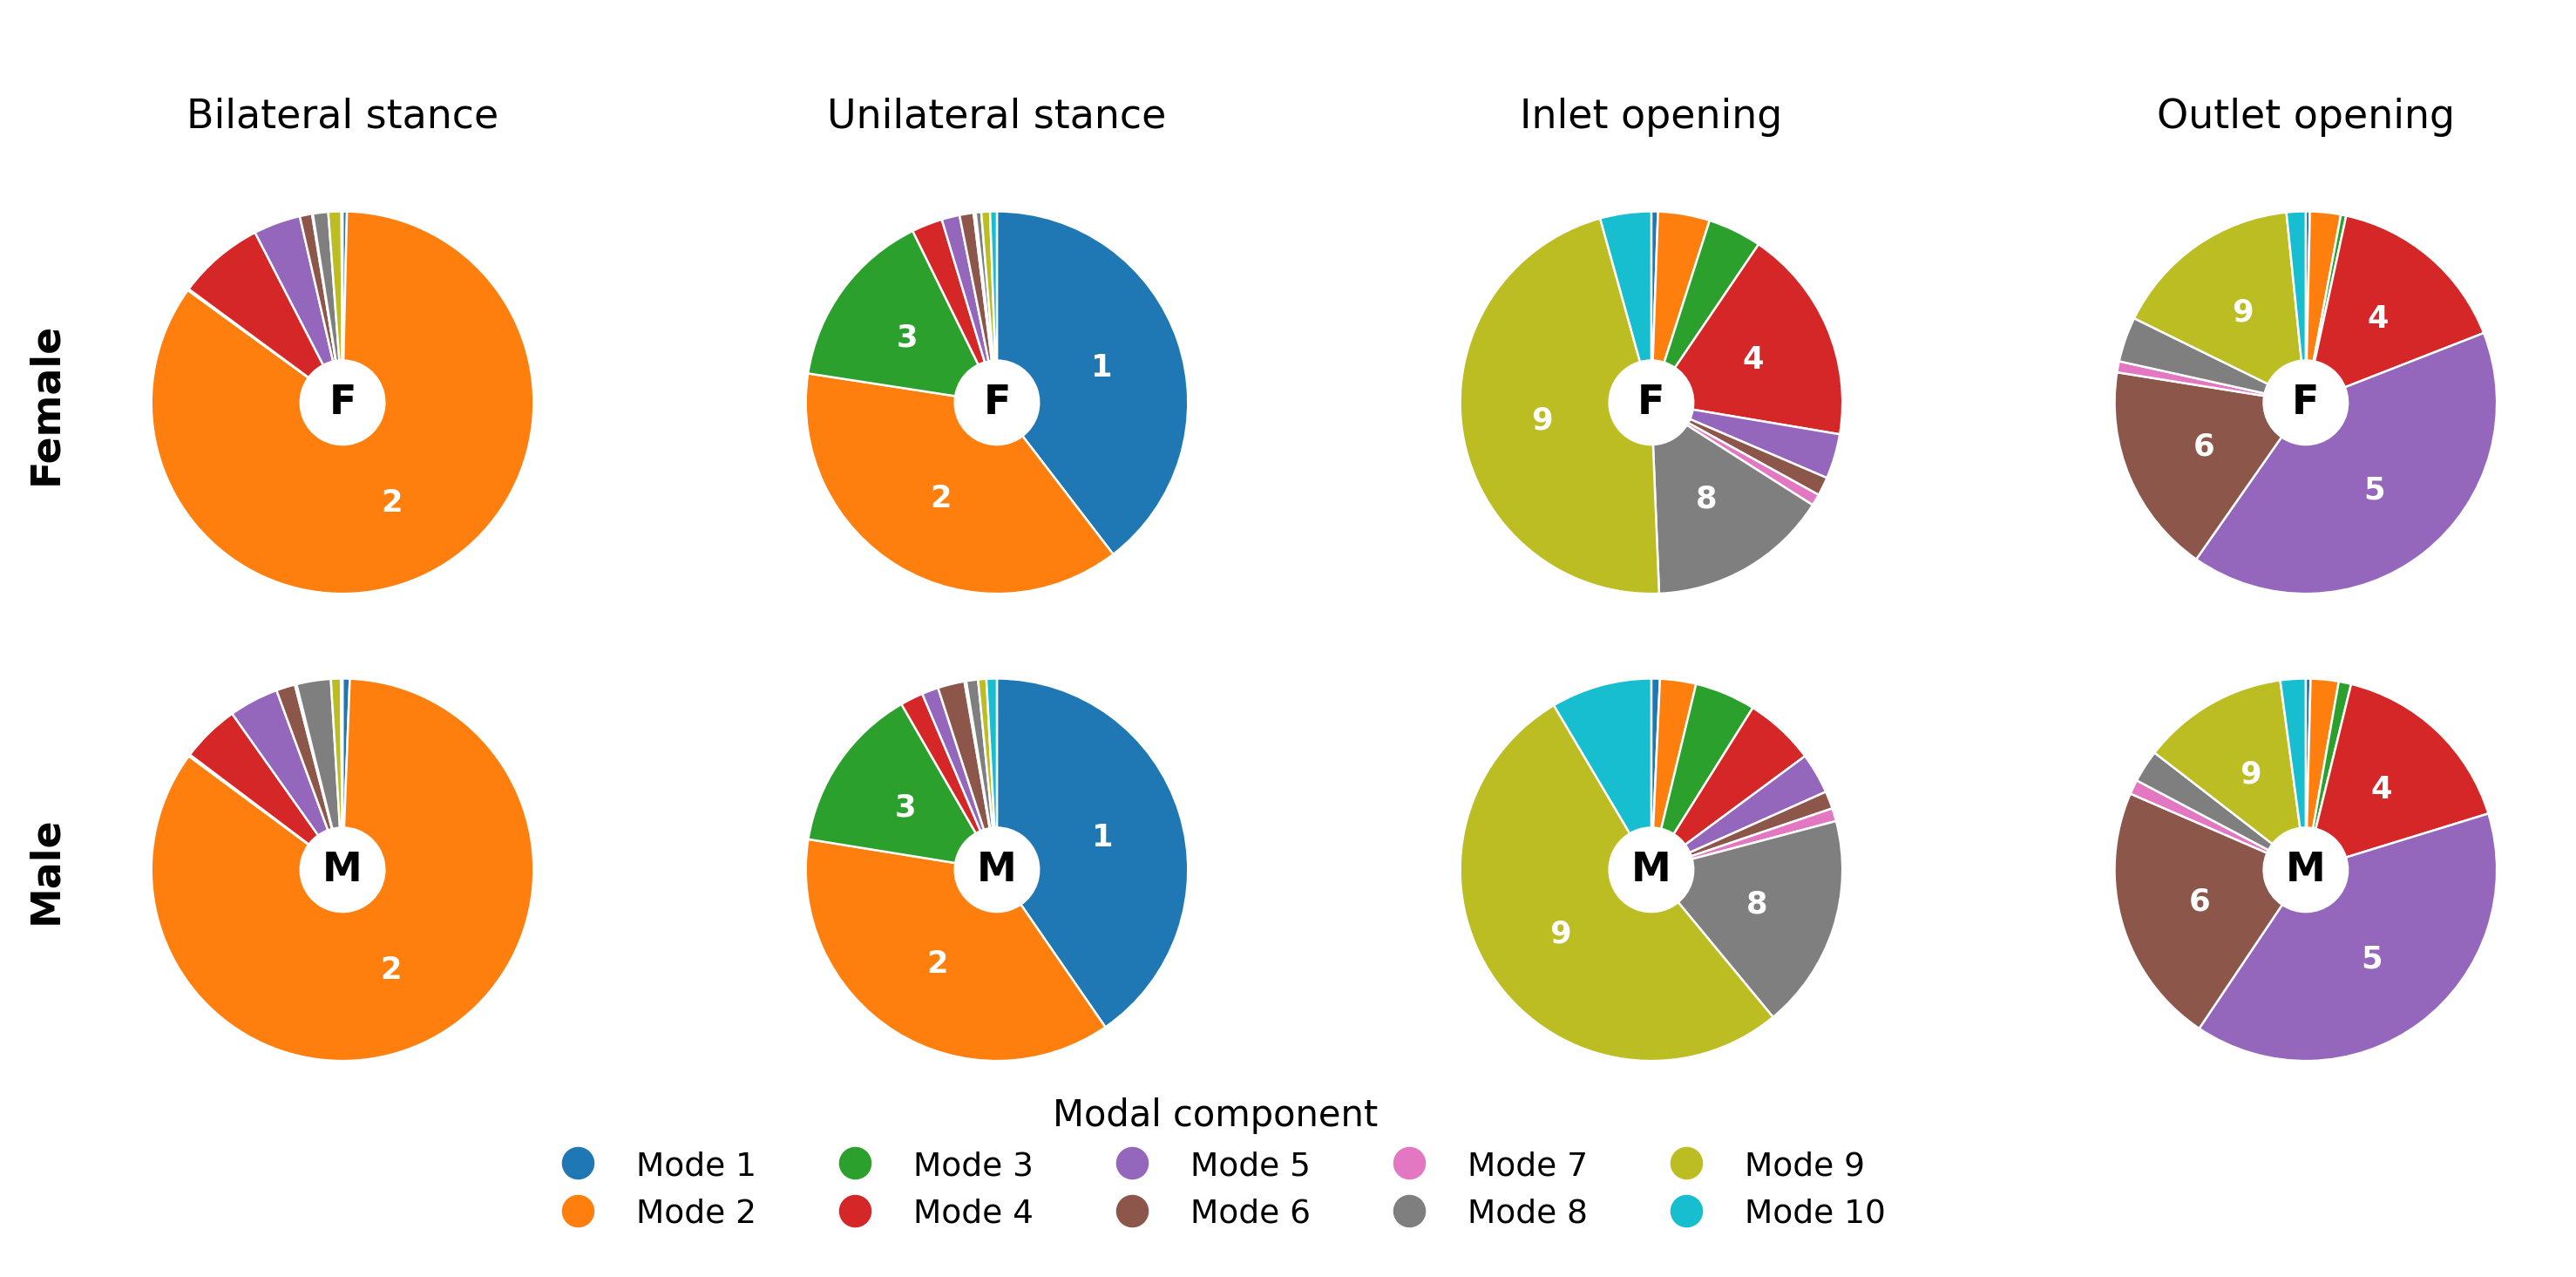
\includegraphics[width=0.95\linewidth]{Figures/Fig3.png}
\caption{Fractional modal decomposition across template-based loading probes. Each small pie chart shows the cohort mean contribution of modes~1--10 to the modal response. Segment colours denote individual modal components (modes~1--10), and labels within selected sectors indicate dominant modes.}
\label{fig:modeshapes}
\end{figure}

\begin{figure}[p]
\centering
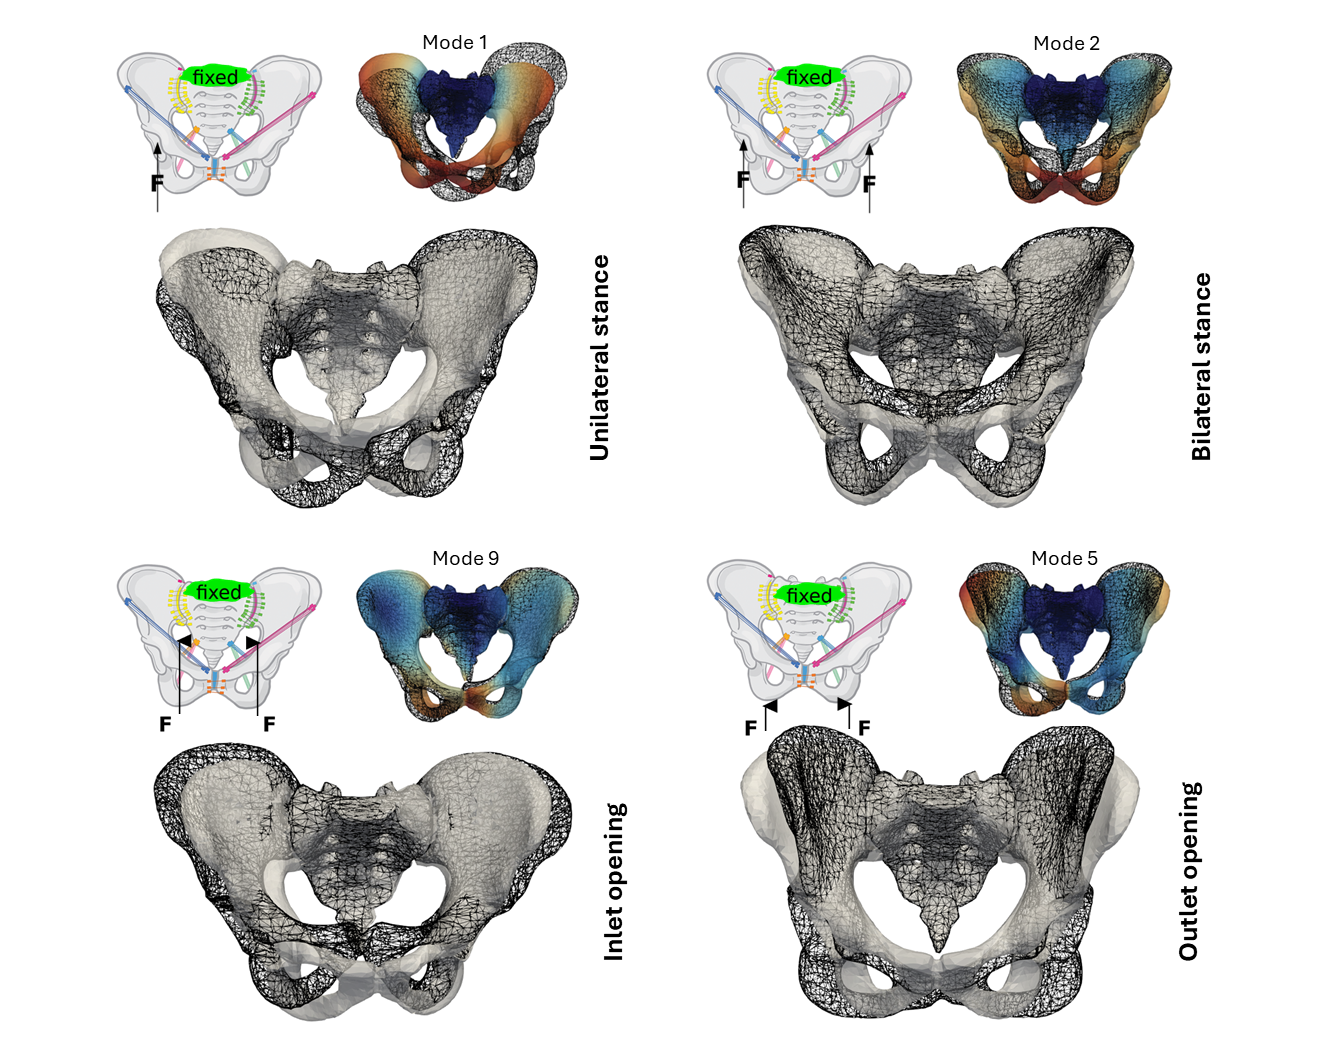
\includegraphics[width=0.95\linewidth]{Figures/Fig6.png}
\caption{Representative modal deformation patterns are shown for each template-based loading probe. Insets indicate the corresponding load application and the most strongly recruited mode, while wireframe overlays illustrate the dominant deformation pathway.}
\label{fig:workflow}
\end{figure}


\clearpage
\printbibliography

\end{document}
